\newpage

% Let us now take a look at generating random values for the $\text{Be}(\alpha, \beta)$ distribution.

\section{Can we apply the inverse transform method to sample random values of a beta distribution? If yes, explain and implement the algorithm. Simulate 15,000 values of a $\text{Be}(3, 9)$ distribution. If no, explain why not.}

\subsubsection*{Applicability to the Beta distribution}

The inverse transform method is a fundamental technique to sample random variables from a given distribution using its CDF. It is based on the fact that if \( U \sim \mathcal{U}[0, 1] \) and \( F \) is a continuous CDF, then the random variable $X = F^{-1}(U)$ has distribution \( F \).

For a \(\text{Be}(\alpha, \beta)\) distribution, the CDF is given by the regularized incomplete Beta function:
\begin{equation}
F(x; \alpha, \beta) = \frac{1}{B(\alpha, \beta)} \int_0^x t^{\alpha - 1}(1 - t)^{\beta - 1} dt
\end{equation}

Although the Beta CDF is smooth and strictly increasing on the interval \([0,1]\), it does not have a closed-form inverse for arbitrary \(\alpha\) and \(\beta\). This means that analytically inverting \(F\) to find \(F^{-1}\) is not feasible.

However, in practice, numerical algorithms can approximate \(F^{-1}\) to a high degree of accuracy. Scientific libraries such as \texttt{scipy.stats.beta.ppf} in Python implement this inverse CDF, referred to as the PPF. The PPF satisfies $F\big(F^{-1}(p)\big) = p$, with $p \in (0,1)$. This allows us to generate Beta-distributed random variables by transforming uniform random variables via the PPF. The monotonicity and continuity of the Beta CDF guarantee the existence of a well-defined inverse function, ensuring the correctness of this sampling method.

\subsubsection*{Simulation and results}

The inverse transform sampling procedure implemented is as follows:
\begin{enumerate}
    \item Generate \(U_1, U_2, \dots, U_{15000} \sim \mathcal{U}[0, 1]\).
    \item Compute \(X_i = F^{-1}(U_i)\) using the Beta quantile function.
    \item Return the sample \(\{X_1, \dots, X_{15000}\}\).
\end{enumerate}

\begin{figure}[H]
    \centering
    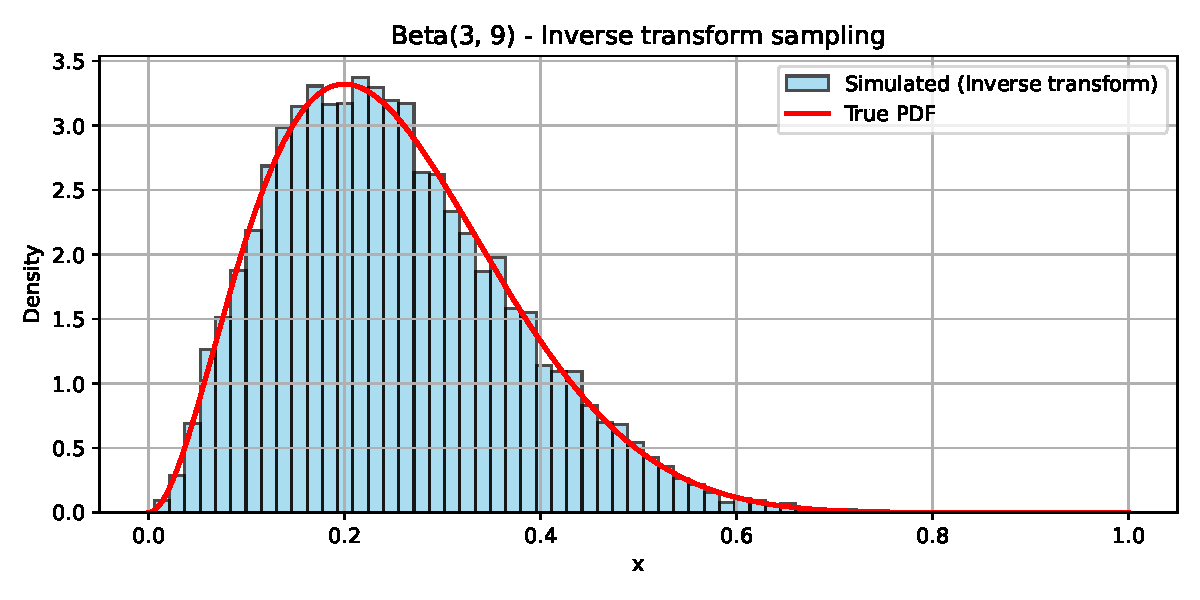
\includegraphics[width=0.7\textwidth]{resources/figures/q2-beta_inverse_transform_sampling.pdf}
    % \caption{Histogram of 15,000 samples from \(\text{Be}(3, 9)\) using inverse transform sampling (blue) compared to the true density (red).}
    \noskipcaption{Histogram of 15,000 samples from \(\text{Be}(3, 9)\) using inverse transform sampling.}
    \label{fig:q2-beta_inverse}
\end{figure}

Figure~\ref{fig:q2-beta_inverse} illustrates that the histogram of generated values aligns closely with the true Beta(3, 9) probability density function. This confirms that the numerical inverse transform method is a valid and practical approach to sampling from Beta distributions.

% \subsubsection*{Remark}

% This approach contrasts with cases such as the exponential distribution, where the inverse CDF is known analytically, enabling direct inversion. For distributions lacking closed-form inverses like the Beta, numerical inversion methods make the inverse transform technique broadly applicable and efficient.





% The inverse transform method is a general technique to sample random variables from a given distribution using its cumulative distribution function (CDF). The principle is based on the fact that if $U \sim \mathcal{U}[0, 1]$ and $F$ is a CDF, then the random variable $X = F^{-1}(U)$ follows the distribution with CDF $F$.

% \subsubsection*{Applicability to the Beta distribution}

% For a $\text{Be}(\alpha, \beta)$ distribution, the CDF is given by the regularized incomplete Beta function:
% \[
% F(x; \alpha, \beta) = \frac{1}{B(\alpha, \beta)} \int_0^x t^{\alpha - 1}(1 - t)^{\beta - 1} dt.
% \]
% However, this CDF does not have a closed-form inverse for arbitrary values of $\alpha$ and $\beta$. Therefore, from a purely analytical standpoint, the inverse transform method is not feasible for the Beta distribution.

% On the other hand, in practice, we can approximate the inverse CDF numerically using scientific libraries such as \texttt{scipy.stats.beta.ppf} in Python. This allows us to apply the inverse transform method computationally, even without a symbolic expression for the inverse.

% \subsubsection*{Simulation and results}

% We used \texttt{scipy.stats.beta.ppf} to apply inverse transform sampling and simulate 15,000 random values from a $\text{Be}(3, 9)$ distribution. The steps are:

% \begin{enumerate}
%     \item Generate $U_1, U_2, \dots, U_{15000} \sim \mathcal{U}[0, 1]$.
%     \item Compute $X_i = F^{-1}(U_i)$ using the beta quantile function.
%     \item Return the sample $\{X_1, \dots, X_{15000}\}$.
% \end{enumerate}

% \begin{figure}[H]
%     \centering
%     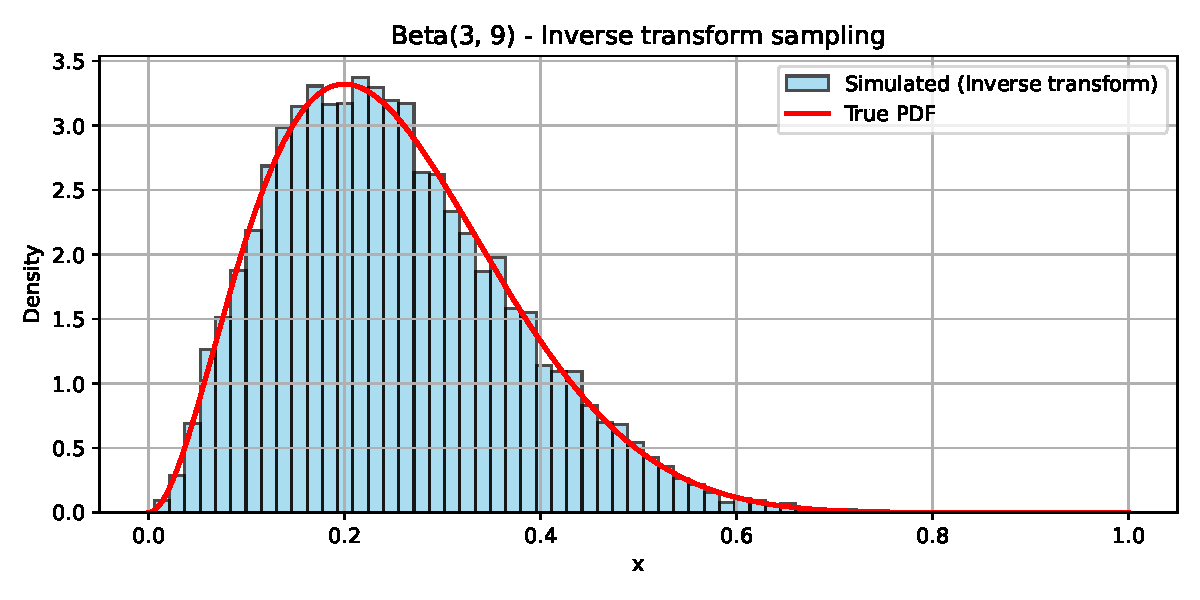
\includegraphics[width=0.7\textwidth]{resources/figures/q2-beta_inverse_transform_sampling.pdf}
%     \caption{Histogram of 15,000 samples from $\text{Be}(3, 9)$ using inverse transform sampling (blue) compared to the true density (red).}
%     \label{fig:q2-beta_inverse}
% \end{figure}

% As shown in Figure~\ref{fig:q2-beta_inverse}, the histogram of the generated values aligns well with the true probability density function of the $\text{Be}(3, 9)$ distribution, confirming the validity of the numerical inverse transform method in practice.

% \subsubsection*{Conclusion}

% Therefore, although the Beta distribution does not have an analytically invertible CDF, we can still apply inverse transform sampling by using numerical approximations. This provides a reliable and efficient method for generating samples, as demonstrated with the $\text{Be}(3, 9)$ simulation.




% ---

% The inverse transform sampling method consists in using the fact that a random variable $X$ with a CDF $F_X$ and $Z = F_X(X)$. We then use the inverse CDF $F_X^{-1}$ to generate $X$ from $Z$, which is uniformly distributed between 0 and 1. 

% In practice, this method is hard to implement because it only applies when the cumulative distribution functions are \textit{explicitly} available. For the beta distribution, finding an explicit expression for the inverse CDF is very hard because of the beta function. Indeed, the CDF of a beta distribution cannot be decomposed in elementary antiderivative form.
